\begin{figure}[h]
    \centering
    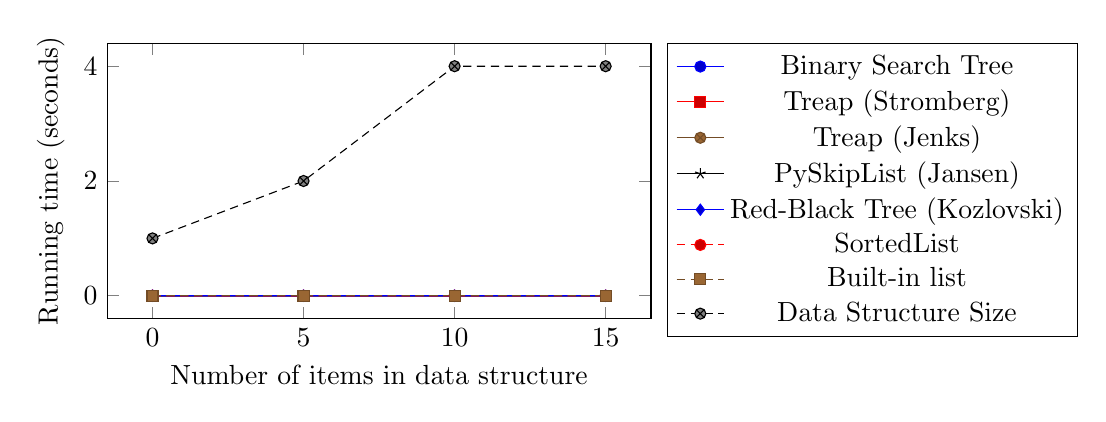
\begin{tikzpicture}
        \begin{axis}[
            xlabel={Number of items in data structure},
            ylabel={Running time (seconds)},
            title={},
            width=0.7\textwidth,
            height=2in,
            legend pos=outer north east
        ]
		\addplot coordinates {
			(0, 3.915279377771754e-06)
			(5, 2.7105780307650593e-06)
			(10, 2.4094026940133903e-06)
			(15, 2.7105780307650593e-06)
		};
		\addplot coordinates {
			(0, 5.722331398281788e-06)
			(5, 5.822723177199023e-06)
			(10, 5.521547840447354e-06)
			(15, 4.919197166944015e-06)
		};
		\addplot coordinates {
			(0, 7.3285998609573695e-06)
			(5, 6.425073850702362e-06)
			(10, 5.822723177199023e-06)
			(15, 4.216454714523405e-06)
		};
		\addplot coordinates {
			(0, 1.0340353228474134e-05)
			(5, 1.1645446354398046e-05)
			(10, 9.336435439301927e-06)
			(15, 8.432909429046884e-06)
		};
		\addplot coordinates {
			(0, 9.637610776053561e-06)
			(5, 9.336435439301856e-06)
			(10, 7.73016697662631e-06)
			(15, 1.0842312123060237e-05)
		};
		\addplot coordinates {
			(0, 4.216454714523442e-06)
			(5, 3.714495819937194e-06)
			(10, 4.216454714523442e-06)
			(15, 4.417238272357912e-06)
		};
		\addplot coordinates {
			(0, 1.4054849048411473e-06)
			(5, 1.30509312592384e-06)
			(10, 1.5058766837583101e-06)
			(15, 1.5058766837583101e-06)
		};
		\addplot coordinates {
			(0, 1)
			(5, 2)
			(10, 4)
			(15, 4)
		};
        \legend{Binary Search Tree, Treap (Stromberg), Treap (Jenks), PySkipList (Jansen), Red-Black Tree (Kozlovski), SortedList, Built-in list, Data Structure Size}
        \end{axis}
    \end{tikzpicture}
    \caption{Average of 3 operations, benchmarked every 5, starting at 0.}
\end{figure}